%%%%%%%%%%%%%%%%%%%%%%%%%%%%%%%%%%%%%%%%%%%%%%%%%%%%%%
%
% This file defines the style for your report
% You don't need to edit it any more, if not to change the authors name.
%
% Search below for the keyword:   GROUP
% insert your group number
%
% Search below for the keyword:   AUTHORS
% insert the name of the authors
%
% If you want to compile your document you have TWO ways
% depending on the fact that 
% 	1) you have inserted only postscript images in your .tex file 
%		---> then go to MODE 1
%	2) you have inserted other kind of images (jpg, pdf, ...) in your .tex file
%		---> then go to MODE 2
%
% MODE 1 
% Type:
% 	latex homebook.tex
%
% If the compilation runs successfully and you want to see the results type:
% 	xdvi homebook.dvi &
% and use the menus to go through the document
%
% If you want to create a pdf type:
% 	dvipdfm homebook.dvi
%
% a homebook.pdf file is created
% you can see it using the command:
% 	acroread homebook.pdf &
%
%
% MODE 2
% Type:
%	pdflatex homebook.tex
%
% If the compilation runs successfully you directly have the pdf file
% and you can see it using the command:
%       acroread homebook.pdf &
%
% 
%%%%%%%%%%%%%%%%%%%%%%%%%%%%%%%%%%%%%%%%%%%%%%%%%%%%%%

\documentclass[10pt,  english, makeidx, a4paper, titlepage, oneside]{book}
\usepackage{babel}
\usepackage{fancyhdr}
\usepackage{makeidx}
\usepackage{titlesec}
\usepackage{listings}
\usepackage{booktabs}

\newenvironment{listato}{\footnotesize}{\normalsize }

%\pagestyle{empty}

\textwidth 15.5cm
\textheight 23cm
\topmargin -1cm
\oddsidemargin -0.5cm
\linespread{1.1}

\pagestyle{fancy}
\lhead{}
\chead{Microelectronic Systems}
\lfoot{}
\cfoot{}
\rfoot{}
\rhead{\thepage}

\usepackage{graphicx}
\usepackage{amsmath}
\usepackage{amsfonts}
\usepackage{amsthm}
\usepackage{amssymb}
%\oddsidemargin -1.1cm
\usepackage{graphicx}
\usepackage{caption}
\usepackage{float}
\usepackage{amsmath}
\usepackage{amssymb}
\usepackage{amsfonts}
\usepackage{amsthm}
%\usepackage{subscript}
\usepackage{empheq}
\usepackage{verbatim}
\usepackage{fancyvrb}

\lstdefinelanguage{VHDL}{morekeywords={library,use,all,entity,generic, is,port,in,out,end,architecture,of,begin,and,if,then,else,elsif,process},morecomment=[l]--}

\lstdefinestyle{vhdl}{language = VHDL, basicstyle = \ttfamily, keywordstyle = \color{keyword}\bfseries, commentstyle = \color{comment}}

\titleformat{\chapter}[display]
{\normalfont\Large\filcenter\sffamily}
{\titlerule[0.5pt]%
\vspace{1pt}
\titlerule
\vspace{1pc}
\LARGE\MakeUppercase{\chaptertitlename} \thechapter
}
{1pc}
{\titlerule
\vspace{1pc}
\Huge}

\makeindex

\begin{document}

\frontmatter
\begin{titlepage}
\vspace{0cm}
\centerline{

\includegraphics[width=3cm]{./logopoli}} 
\vspace{0.5cm}
\centerline{\LARGE Politecnico di Torino}
\vspace{2.5cm}
\centerline{\huge\sf Integrated Systems Architectures}
\vspace{1cm}
\centerline{\Huge\sf Laboratory 1}
\bigskip
\centerline{\huge\sf Design and implementation of a digital filter}
\vspace{2cm}
\centerline{\Large Master degree in Electronics Engineering}
\bigskip
\centerline{\Large Master degree in Computer Engineering}
\vspace{4.5cm}
%%%%%%%%%%%%%%%%%%%%%%%%%%%%%%%%%%%%%%%%%%%%%%%%%%%%%%
%
\centerline{\large Referents: Prof. Guido Masera}
\bigskip
\vspace{1cm}
%
%%%%%%%%%%%%%%%%%%%%%%%%%%%%%%%%%%%%%%%%%%%%%%%%%%%%%%
% GROUP
% Change the name of your group below
%
\centerline{\large Authors: group\_21}
\bigskip
%
%%%%%%%%%%%%%%%%%%%%%%%%%%%%%%%%%%%%%%%%%%%%%%%%%%%%%%
% AUTHORS
% Change the name of the Group participants here
%
\centerline{\large Nicola Dilillo, Stefano Moncalvo, Lorenzo}
%
%%%%%%%%%%%%%%%%%%%%%%%%%%%%%%%%%%%%%%%%%%%%%%%%%%%%%%
\vspace{2cm}
\centerline{\large \today}
\end{titlepage}

\tableofcontents

\mainmatter
%%%%%%%%%%%%%%%%%%%%%%%%%%%%%%%%%%%%%%%%%%%%%%%%%%%%%%
%    
% HERE IS WHERE YOU INCLUDE YOUR CHAPTERS
%
%%%%%%%%%%%%%%%%%%%%%%%%%%%%%%%%%%%%%%%%%%%%%%%%%%%%
% This will help you in writing your homebook
% Remember that the character % is a comment in latex
%
% chapter 1
\chapter{Prototype}
\label{chap1}
%%\graphicspath{ {./chapters/chap1images/} }
%%%%%%%%%%%%%%%%%%%%%%%%%%%%%%%%%%%%%%%%%%%%%%%%%%%%%%%%%%%
% you can organize a chapter using sections -> \section{Simulating an inverter}
% or subsections -> \subsection{simulating a particular type of inverter}
%%%%%%   First section
\section{Introduction}
In order to better and easier simulate the architecture, two scripts have been used:
A bash script to control the simulation from high level: it is in charge to invoke the C script with the right command line argument during the proper simulation phase and to 
run modelsim;
A C script in charge to perfrom various operations during different steps of the simulation, manipulating different files.
For simplicity, a single value is assigned to both operands each simulation cycle, de facto using the multiplier as a square-evaluation circuit.
\section{General simulation flow}
The C script can accepts an additional command line parameter:
-i corresponds to TEST\_INIT mode: the script reads the handwrittensamples.txt file, in which desired inputs in human-like format are stored, e.g. 12.29487, -0.9872 etc, 
and generates two other files as output, both storing data in hexadecimal encoding:
simulationinputs.hex, which contains the inputs for the Modlesim simulation
expected\_outputs.hex, which contains the outputs that are expected to be generated by the Modelsim simulation.
-v corresponds to TEST\_VALIDATION mode: the script executes a diff command between the self-generated expected\_outputs.hex file and the file generated by the Modelsim simulation using 
a pipe to execute it in background and take back its output, then processing it in order to establish if the two files are identical, Test Successful, or different, Test Failed.
The flow of the simulation is the following:
-the bash script executes the C program passing -i as command line parameter in order to generate the input vectors for the simulation and the file storing the expected results.
-Modelsim is launched and the effective output file is generated
-the C program is executed passing -v as command line parameter in order to compare the simulation results with the expected ones

\section{C script}
Since IEEE754 is the standard encoding that is normally used to store floating point data inside a flash memory, to convert a floating point value in its equivalent hexadecimal 
encoding it's sufficient to use the   \textbf{union}  C data type.
\textbf{union} data type allows to store multiple-encoding data variables in the same memory location, thus it is sufficient read a value from the handwrittensamples.hex file 
and store it as a float variable inside the previously declared memory location, and then accessing it using the other encoding
\begin{lstlisting}[style=CStyle]
    union IEEE754conv 
    {
        float f;
        uint32_t ieee754Value;
    };

\end{lstlisting}

The previously described operation is trivially implemented by the following procedure, that is very convenient both in terms synthax and in terms of CPU time, since what is done is just a couple of memory accesses:
\begin{lstlisting}[style=CStyle]
    uint32_t convFloatinIEEE754(float val)
    {
            union IEEE754conv conv;
            conv.f = val;
            return conv.ieee754Value;
    }
\end{lstlisting}

%%%%%%%%%%%%%%%%%%%%%%%%%%%%%%%%%%%%%%%%%%%%%%%%%%%%
% This will help you in writing your homebook
% Remember that the character % is a comment in latex
%
% chapter 2
 
\chapter{Datapath}
\label{cha2}
\section{Fetch Stage}
During fetch stage, an instruction is read from the instruction register accordingly to the content of the Program Counter, a 32-bit register that stores the address 
of the next instruction to be fetched. Fetched instructions are then passed to the next stage.
Assuming the case of the execution of concurrent instructions, from one instruction to the next one the program counter is incremented by 4. This is because each instruction 
is encoded on 4 bytes and the instruction memory is byte-addressed, thus we have an offset of 4 bits.
In case of branch instructions or jumps, the value of the program counter can be modified in other ways using various offsets and rules depending on the case, 
as it will discussed later.

\begin{figure}[!h]
    \centering
        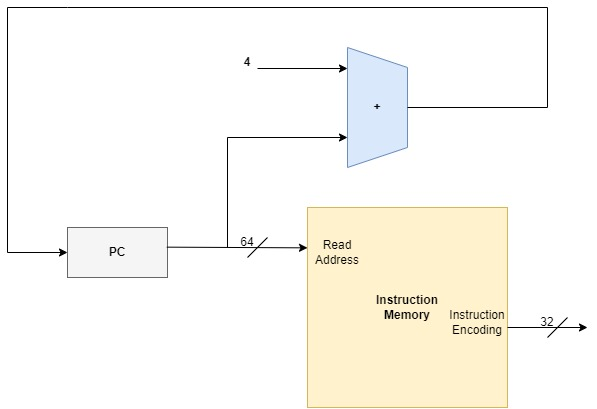
\includegraphics[width=\linewidth]{schematic/InstructionMemory_withProgramCounter.jpg}
        \caption{\textbf{Instruction Format}}
\end{figure}
    

\section{Decode Stage}

In decode stage the instruction that has been previously fetched is decoded by means of the bit-fields that compose it.
Operands are decoded, be them a content of a register or an immediate value, and the control bits for the other components eventually employed in requested calculation 
(e.g. multiplexers or the ALU) are prepared to be sent to next stage through pipeline. In this stage stall or nope can be 
added due to a data hazards or a branch instruction. This behavior is better explained in the dedicated section.

\subsection{Register File}

The register file stores internal runtime values used during calculations.
Some registers have specific purposes, such as the stack pointer, the thread pointer, the return address or the register r0, the only one that can't be overwritten 
and that always stores a value of all zeros; other registers can be used during program execution, and are said to be \textbf{general purpose registers}.
The register file is synchronous with the falling edge of the clock signal and it is composed by a total of 32 registers, indexed by means of 5-bit address lines.
It has been decided to keep the register file always able to provide data in reading, without any enable signal, while a dedicated signal is needed to allow writing operations.
An active-high reset signal is present, in order to clear the entire content of the registers.

\begin{figure}[!h]
    \centering
        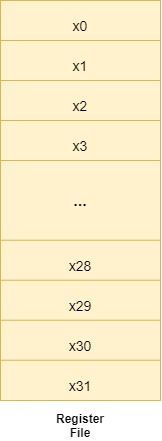
\includegraphics[width=0.2\linewidth]{schematic/RegisterFile.jpg}
        \caption{\textbf{Register File}}
\end{figure}
    
Register File is composed of two read data port, able to access two sources at the same time, and one write data port.

\clearpage

\subsection{Immediate generator}

When an instruction containing an immediate occurs this value must be extrapolated, and different opcodes require 
different ways to compose it. The immediate must be computed on 32 bits.

\section{Execute Stage}

During the execute stage, operands are sent to the ALU in order to perform the required computation. 
The operand can be provided from different stages of the pipeline and a specific unit is in charge of feeding ALU with the right value.

\subsection{ALU}

The Arithmetic Logic Unit is the computational core of the overall architecture.
Since we chose to support 32 bits of parallelism for registers and data management, the ALU has been built with a parallelism of 32 bits too.
The Arithmetic Logic Unit has been developed by means of standard arithmetic operations, implemented with behavioral VHDL language, in order to allow the compiler 
to have a certain freedom during optimization.
To better manage constants, sizes and opcodes, all meaningful values have been declared in the file \textit{myTypes.vhd}.
The ALU is implemented using a process, in which inputs are employed into the proper computation by means of a control signal on 3 bits.
Since the control unit is an hardwired one, this control signal is directly derived from original opcode of the decoded instruction.
The operations that ALU can perform are:
\begin{itemize}
    \item addition, sum operand A and B;
    \item addition PC, sum 4 to operand A;
    \item arithmetic shift to right, arithmetic shift operant A to right of position number equal to B;
    \item absolute function, elaborate the absolute value of operand A and add B to it;
    \item and, execute AND operation, bit by bit, between operand A and B;
    \item or, execute OR operation, bit by bit, between operand A and B;
    \item xor, execute XOR operation, bit by bit, between operand A and B.
\end{itemize}
    

\subsection{Absolute Module}

An entity has been written in order to allow the computation of absolute value of an integer register.
This module has two input ports and one output ports. The value on the first input port is the one to convert 
through the absolute function. To achieve this result it sees the last bit of the signal if a zero is detected 
no operations are performed, while if a 1 is detected all the bits are complemented and is added a one. 
These are the steps to covert a number, in this case from a negative to a positive value, according absolute function.
At the end the second input is summed to the convert one and the result is sent to the output.
This component has been inserted into the ALU to increase its operational capacity.

\subsection{Forwarding Unit}

Forwarding Unit is a component with an important purpose: forward a previously computed result to one of the ALU inputs
before it is effectively written in register file, in order to resolve a possible Data Hazard, avoiding a stall.
The need to forward a certain value in one of the stages following the Execution one is detected by means of comparison between the encodings of the source registers 
that are passed from Decode stage to the Execute Stage, and the encodings that are actually kept in Memory and Write-back stages.
If an equivalence is found, this means that the instruction that has been decoded in previous clock cycle is asking as operand a result that is not yet available 
in register file, but that has already been computed, thus it is possible to directly wire it to the proper ALU input via additional interconnections
couple of multiplexer, as shown in figure.  

Forwarding for multiplexer A is based also on the possibility to pick the value of Program Counter, it takes care about \textit{ALUSrc\_PC} signal.
While the output of multiplexer B is the input of another one that chooses between the source register and the immediate value, the decision is 
taken through the control signal \textit{ALUSrc}. 

\begin{figure}[!h]
    \centering
        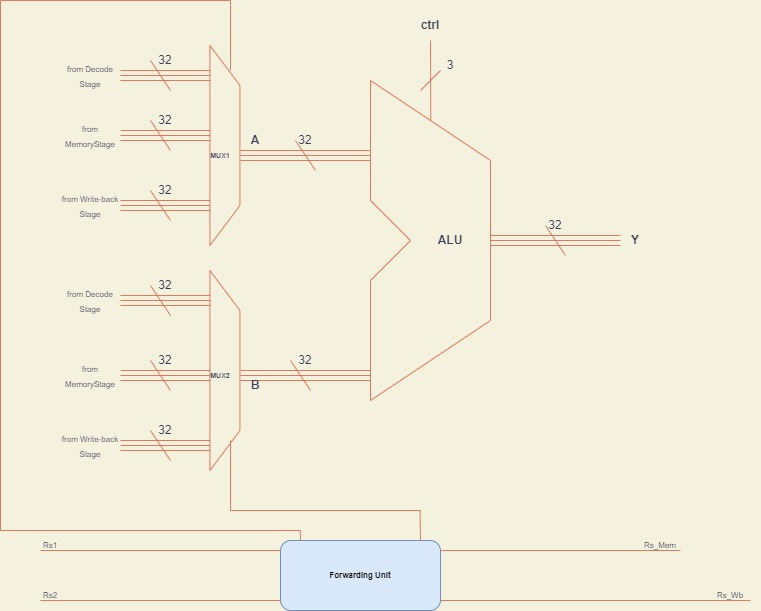
\includegraphics[width=\linewidth]{schematic/ALUwithForwardingUnit.jpg}
        \caption{\textbf{ALU with Forwarding Unit}}
\end{figure}
    

\section{Memory Stage}

Memory stage is the step of the pipeline in which results are loaded/stored in the main memory.
The memory is byte addressed and characterized to be Little Endian, i.e. the least significant byte is stored at a least address than the most significant one.
The main memory is involved in load and store operations, that directly invoke it. It has a crucial role during when composite data need to be stored to guarantee 
the program correctness.
Since RISCV does not require stored words to be aligned in memory, their management is simpler and requires less hardware resources.

\section{Write Back Stage}

During Write-back stage, the register file is accessed in order to store the result of the previously performed calculation inside the destination register,
determined during the past decoding phase of the instruction that has generated this value.
As previously clarified, the register file needs in this case that the relative write-enable signal is set in order to be able to accept a new value inside one 
of its locations, and the control unit is in charge of properly drive that enable signal.
%%%%%%%%%%%%%%%%%%%%%%%%%%%%%%%%%%%%%%%%%%%%%%%%%%%%
% This will help you in writing your homebook
% Remember that the character % is a comment in latex
%
% chapter 3
\chapter{Advanced architecture development}
\label{cha3}

In this section the purpose is to improve the FIR performance. In first and unfolding 
technique has been used to improve the throughput and then pipeline technique has 
been used to reduce the longest path and improve maximum frequency.

\section{Unfolding}

Unfolding of order 3 has been applied to FIR filter (N = 3) and the equations derived
to build the new system are the following:

\begin{equation}
\begin{split}
    y[3n] = a_0 \cdot x[3n] + a_1 \cdot x[3(n-1) + 2] + a_2 \cdot x[3(n-1) + 1] + \\
    a_3 \cdot x[3(n-1)] + a_4 \cdot x[3(n-2) + 2] + a_5 \cdot x[3(n-2) + 1] + a_6 \cdot x[3(n-2)] +  \\
    a_7 \cdot x[3(n-3) + 2] + a_8 \cdot x[3(n-3) + 1] + a_9 \cdot x[3(n-3)] + a_{10} \cdot x[3(n-4) + 2]
\end{split}
\end{equation}

\begin{equation}
\begin{split}
    y[3n + 1] = a_0 \cdot x[3n + 1] + a_1 \cdot x[3n] + a_2 \cdot x[3(n-1) + 2] + \\
    a_3 \cdot x[3(n-1) + 1] + a_4 \cdot x[3(n-1)] + a_5 \cdot x[3(n-2) + 2] + a_6 \cdot x[3(n-2)+1] +  \\
    a_7 \cdot x[3(n-2)] + a_8 \cdot x[3(n-3)+2] + a_9 \cdot x[3(n-3) + 1] + a_{10} \cdot x[3(n-3)]
\end{split}
\end{equation}

\begin{equation}
\begin{split}
    y[3n + 2] = a_0 \cdot x[3n + 2] + a_1 \cdot x[3n + 1] + a_2 \cdot x[3n] + a_3 \cdot x[3(n-1) + 2] +\\
    a_4 \cdot x[3(n-1) + 1] + a_5 \cdot x[3(n-1)] + a_6 \cdot x[3(n-2) + 2] +  a_7 \cdot x[3(n-3) + 1] +\\
    a_8 \cdot x[3(n-2)] + a_9 \cdot x[3(n-3) + 2] + a_[10] \cdot x[3(n-3) + 1]
\end{split}
\end{equation}

Using this method of optimization the two more input and output port have been added becouse
now 3 inputs are processed and produce, at the same time, 3 output. To overall throughput has
been triplicate.

%% formula dove facciamo vedere che il throuput è triplicato e il nuovo valore calcolato

\section{Pipeline}

A further optimization has been applied. This method allows to reduce the size of critical path.

From schematic of previous FIR is possible to see that the critical path is the chain off 
adders. To achieve the best result is not necessary split each of them, but it is needed to 
group them in order to have a total time path that is less than the amount of time for performed
a multiplication. 


% \input{./chapters/chap_name}
% and so on
%
%%%%%%%%%%%%%%%%%%%%%%%%%%%%%%%%%%%%%%%%%%%%%%%%%%%%%%
%    
% HERE IS WHERE YOU INCLUDE YOUR APPENDICES (IF ANY)
%
%\appendix
%%%% Appendix A
\chapter{Adder behavioural VHDL}
\label{appendix1}

	\lstinputlisting[language=VHDL, breaklines=true]{appendices/files/adder.vhd}

% \lstinputlisting is an alternative way to import text or code from an external file. In this example the behavioural VHDL description of an adder contained in the file adder.vhd is imported. 
% Note that you can set the language of the code that you want to import (VHDL in this example). When you set the language you will see the keywords of that specific language highlighted in your output pdf file.
%You can set a lot parameters: for some examples take a look at the chapter 'How to document the project' that can you find in DLX_Project.pdf.
%\input{./appendices/appendix2}
% and so on
%
%%%%%%%%%%%%%%%%%%%%%%%%%%%%%%%%%%%%%%%%%%%%%%%%%%%%%%

\end{document}